\section{What moves the effect, and what does not}
\label{sec:analysis}

Section~\ref{sec:results} attributes the inversion to the failed call's surface
form. If that attribution is right, the effect should respond to manipulations
of the \emph{form} and be largely indifferent to manipulations of the
\emph{message}. Table~\ref{tab:probe-manipulations} and
Figure~\ref{fig:manipulations} test exactly that. Every row uses the same items
and the same failing call; only how the failure is written into the transcript
changes.

Throughout this section we report each variant as a \emph{paired} change in
$\log \pi(\afail)$ relative to the standard harness, computed item by item.
Comparing two independently estimated gains would confound the manipulation with
which items each variant happened to be scored on; pairing removes that, and it
also removes item difficulty, which is the dominant source of variance here.
Positive means the variant makes repetition \emph{more} likely.

% Requires in the preamble:
% \newcommand{\ci}[2]{{\scriptsize\,[#1,\,#2]}}

\begin{table*}[t]
\centering
\tblfont
\setlength{\tabcolsep}{\tblsep}
\begin{tabular}{l c c}
\toprule
Harness variant & SmolLM2-135M & Qwen2.5-0.5B \\
\midrule
terse error text & \textminus 0.32\,\ci{\textminus 0.72}{0.02} & \textminus 0.23\,\ci{\textminus 0.64}{0.20} \\
verbose error text & \textminus 0.09\,\ci{\textminus 0.32}{0.14} & \textminus 0.31\,\ci{\textminus 0.65}{0.02} \\
error quotes the failed call & \textbf{1.31\,\ci{1.12}{1.51}} & 0.10\,\ci{\textminus 0.22}{0.44} \\
failure placed before the successful steps & \textbf{\textminus 0.94\,\ci{\textminus 1.45}{\textminus 0.48}} & \textbf{\textminus 0.82\,\ci{\textminus 1.36}{\textminus 0.26}} \\
+ ``do not repeat'' instruction & \textbf{0.16\,\ci{0.06}{0.27}} & \textminus 0.02\,\ci{\textminus 0.20}{0.15} \\
the same call failed twice & \textbf{3.06\,\ci{2.78}{3.36}} & \textbf{3.61\,\ci{3.12}{4.08}} \\
the same call failed three times & \textbf{3.29\,\ci{3.01}{3.59}} & \textbf{4.78\,\ci{4.18}{5.37}} \\
placebo: a \emph{different} call failed & \textbf{\textminus 15.71\,\ci{\textminus 17.38}{\textminus 14.23}} & \textbf{\textminus 11.71\,\ci{\textminus 13.28}{\textminus 10.18}} \\
abstracted failure (no verbatim call) & \textbf{\textminus 21.68\,\ci{\textminus 23.20}{\textminus 20.14}} & \textbf{\textminus 11.05\,\ci{\textminus 12.80}{\textminus 9.39}} \\
\quad bare marker, no diagnosis & \textbf{\textminus 24.23\,\ci{\textminus 26.30}{\textminus 22.32}} & \textbf{\textminus 13.01\,\ci{\textminus 15.04}{\textminus 11.10}} \\
\bottomrule
\end{tabular}
\caption{Harness variants, as \emph{paired} changes in the log-probability of re-emitting the failed call, relative to the standard harness on the same items. Positive means the variant makes repetition \emph{more} likely; negative means less. Every row uses the same items and the same failed call, and only how the failure is written into the transcript changes.}
\label{tab:probe-manipulations}
\end{table*}


\begin{figure}[t]
\centering
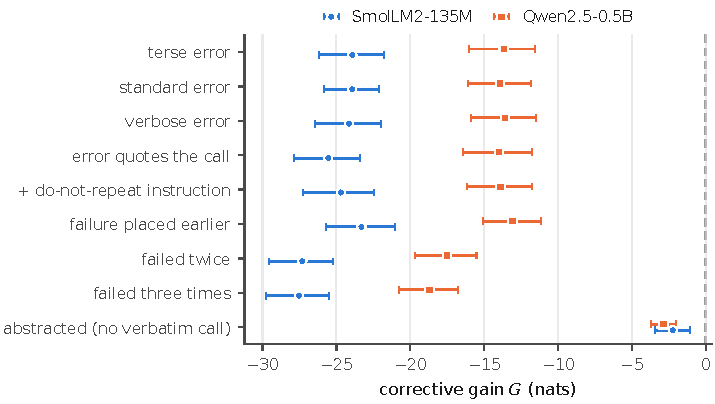
\includegraphics[width=\linewidth]{figures/fig5_manipulations}
\caption{Corrective gain under harness variants. Points right of the dashed line
would mean the failure record suppresses the failed call. Manipulations of the
message (top four rows) move the estimate very little; the manipulation that
removes the call's surface form (bottom row) moves it by an order of magnitude.}
\label{fig:manipulations}
\end{figure}

\paragraph{Message content is nearly inert.}
Shortening the error to a bare category name changes the log-probability of
repeating by \DTerseCI\ nats; expanding it with the tool signature and a
corrective hint changes it by \DVerboseCI. Both intervals contain zero. The
verbose rendering explicitly names the argument the model should have used, which is about as informative
as an error message can be without solving the task, and it does not
measurably move the quantity that decides whether the call gets
written again.

\paragraph{Occurrence count is not inert.}
When the runtime echoes the offending call inside the error message, as a
Python traceback does by default and as several agent frameworks do by
convention, the failed call appears twice instead of once, and repetition
becomes \DEchoCI\ nats more likely. The interval excludes zero. Set against
the near-zero effect of rewriting the message, this is the sharpest contrast we
have between form and content: adding information changes nothing, adding a
second copy of the string changes something.

It is also a small, actionable finding on its own. A runtime that helpfully
quotes back what you tried is, for a small model, making the situation slightly
worse.

\paragraph{Repetition compounds.}
When the same call fails twice the effect grows by \DTwiceCI\ nats, and three
times by \DThriceCI. That is the situation an agent is already in by the time
anyone notices it is stuck, and each additional failure digs the hole deeper.
This is the self-reinforcement of \citet{xu2022breaktheloop} operating inside an
agent trajectory, with the difference that here an explicit corrective signal is
present at every repetition and does not arrest it.

\paragraph{Recency is not the explanation.}
Moving the failed step to \emph{before} the successful prefix steps, so that it
is no longer the most recent thing in the transcript, helps by \DEarlyCI\ nats, a real effect and about three percent of the
total. Whatever is happening
is not simply the last turn dominating.

\paragraph{Telling the model not to repeat does not help.}
Adding a system-prompt instruction not to repeat a call that has already failed
changes the log-probability of repeating by \DInstructionCI\ nats. The
instruction is unambiguous, it sits in the same context window, and the model is
instruction-tuned. The effect is small but its sign is the wrong one, which is
what the negative-instruction literature would predict
\citep{castricato2024pinkelephants,negation2025pinkelephant}: a prohibition that
has to name a string cannot easily beat the presence of that string.
Section~\ref{sec:agent} reports the same intervention in free-running rollouts,
where it also fails to reduce repetition, but where it does change behaviour
in a way this measurement does not anticipate.

\paragraph{Removing the surface form does.}
Replacing the verbatim call with a runtime-generated description of the
failure, which keeps the diagnosis and drops the token sequence, moves the
log-probability of repeating
by \DAbstractCI\ nats, which is very nearly the whole effect, and drives the
exact greedy repeat rate to zero for every model
(Table~\ref{tab:probe-repeat-toolshed}). The description is produced
deterministically from the runtime's own error metadata; no additional model
call is involved, so this is a change to the harness, not to the agent.

\subsection{Controls}

\paragraph{A placebo: someone else's failure.}
The strongest version of the ``you have just rediscovered copying'' objection is
that any failure in the context might raise the probability of any plausible
action. We test it directly. In the \emph{fail\_other} condition the transcript
records a \emph{different} plausible-but-wrong call as having failed, with its
own genuine error message; the action we score was never written.

Relative to the standard harness, the placebo recovers \DPlaceboCI\ nats, a large majority of the effect,
but not all of it. The reason it does not
recover all of it is worth being explicit about: the distractor is another
perturbation of the
\emph{same} reference call, so it shares most of its tokens with the action being
scored, and the placebo therefore leaks copying by construction. That makes it a
conservative control rather than a broken one. It bounds the string-specific
component from below at \StringSpecificBound\ nats, and we report it that way
rather than attributing all of $\Gain$ to the exact string. A placebo drawn from
an unrelated call would tighten the bound and is the obvious refinement.

\paragraph{Does the abstraction work because of what it says?}
Our abstraction replaces the call with a short diagnosis, and we wrote those glosses, so perhaps it works because the glosses are good,
which would not generalise. \emph{abstract\_min} strips them: the transcript gets
\texttt{[attempt 1 failed]} and nothing else, no call and no diagnosis. It
recovers \DAbstractMinCI\ nats, against \DAbstractMatchedCI\ for the full abstraction on the same models, if
anything slightly more. The benefit is
the absence of the string, not our wording, which is what the decomposition
predicts and the version of the result that transfers to other runtimes.

That does not make the diagnosis worthless, since it is what the model needs
in order to write a \emph{different} call rather than merely a different
string, but it is not what is doing the work here.

\paragraph{Is the ``neutral'' observation really neutral?}
``Call recorded.'' might read as mildly positive, which would make $\copyterm$
absorb some of what belongs to $\semterm$. Table~\ref{tab:probe-robustness}
therefore repeats the decomposition using the counterfactual \emph{success}
observation as the reference instead. The two references bracket any reasonable
notion of neutrality, and the conclusion should not depend on which is chosen.

\paragraph{Length.}
The failure observation is longer than the valence-free one, so part of
$\semterm$ could be a position effect rather than a content effect. Repeating
the decomposition against a neutral observation padded to the same token length
with valence-free trace identifiers separates the two, and the answer is clean
in both directions. The surface-form term is unmoved, at \MeanCopy\ against a short neutral and
\CopyPad\ against a length-matched one, so the effect the paper rests on is
not an artefact of context length. The semantic term shrinks from
\MeanSem\ to \SemPad, meaning most of the small positive value it had was
indeed position rather than content. What survives is a corrective term of under
a nat, against a surface-form term of more than twenty.

\paragraph{Error family.}
Figure~\ref{fig:error-types} and Table~\ref{tab:by-error} break the gain down by
the kind of error the call provoked. The effect is present in every family; a
result concentrated in one would have suggested that the wording of one error
message, rather than the mechanism we describe, was responsible.

\begin{figure}[t]
\centering
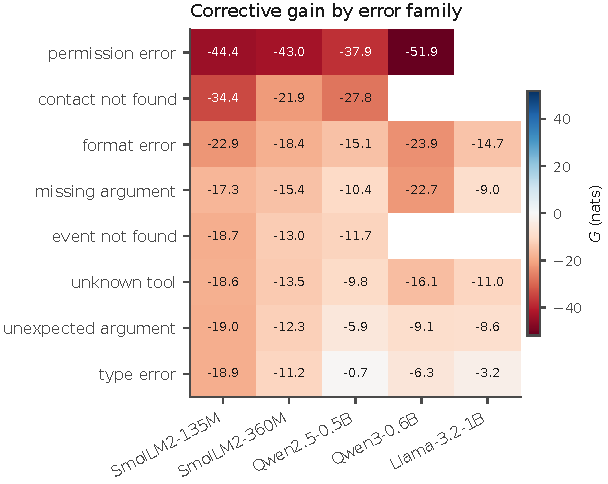
\includegraphics[width=\linewidth]{figures/fig6_error_types}
\caption{Corrective gain by error family (ToolShed), one cell per
model\,$\times$\,family. The scale is diverging about zero, so red is feedback
inversion and blue would be a harness behaving as intended; no cell is blue.
Blank cells are model/family pairs the schedule did not reach.}
\label{fig:error-types}
\end{figure}

\subsection{Does copying just raise everything?}

We return to this because it is the objection a careful reader should raise
twice. Copying from context is indiscriminate, so the correct action, which usually differs from the failed one by a single
argument name or value, should also become more likely, and it does. Three observations keep the result from
collapsing into that.

First, the quantity that governs the agent's next move is the difference, and
the difference moves against the correct action
(Table~\ref{tab:probe-robustness}, $\Delta$margin). Second, the normalised
repeat probability is computed over a fixed candidate set that includes the
correct action and two alternative wrong actions, so a uniform lift cancels out;
it still rises sharply. Third, the greedy readout is a statement about the
argmax, which is immune to uniform lifts by construction: after the failure, the
single most likely continuation \emph{is} the failed call on a large fraction of
items, and before it, on none.
